\section{Socket-Schnittstelle}

Die \textbf{Socket-Schnittstelle} ermöglicht die Kommunikation von verteilten Client-Server-Anwendungen untereinander.\\

\begin{tcolorbox}
Die Socket-Schnittstelle stellt eine Schnittstelle zwischen \textbf{Schicht 4} (Transportschicht) und \textbf{Schicht 5} (Anwendungsschicht) dar.
\end{tcolorbox}

\subsection{Socket-Schnittstelle zu UDP}

Eine Schnittstelle zu \textbf{UDP} ist relativ einfach zu realisieren, da hier keine Operationen für den Verbindungsauf- und -abbau nötig sind $\rightarrow$ es sind nur Operationen für das Senden und Empfangen notwendig.\\

\noindent
Bei der Erzeugung eines \textbf{Sockets} kann eine Portnummer angegeben werden, für gesendete Nachrichten ist das dann die \textbf{Quellportnummer} der Nachricht.\\
Der Socket empfängt nur Nachrichten, die an diesen Port adressiert wurden.\\

\noindent
Bei \textbf{Client/Server-Anwendungen} geht die Initiative vom Client aus, der eine Anfrage an einen Server schickt.\\
Der Server antwortet an die in der Nachricht enthaltenen IP-Adresse und Quellportnummer.

\begin{tcolorbox}
I.d.R verwendet ein Client eine beliebige freie Portnummer.\\

\noindent
Dienste laufen auf Servern auf wohlbekannten Portnummern, bspw. ``https`` auf Port $443$\footnote{
s. a. ``Hypertext Transfer Protocol Secure``: \url{https://de.wikipedia.org/wiki/Hypertext_Transfer_Protocol_Secure} - abgerufen 30.01.2024
}.\\
Ein Server, der unter einer bestimmten Portnummer laufen soll, kann nur gestartet werden, wenn die Postnummer nicht schon belegt ist.
\end{tcolorbox}\\

Beispiel für eine Programmstruktur für eine Kommunikation zwischen UDP-Client und -Server:
\begin{minted}[mathescape,
    linenos,
    numbersep=5pt,
    gobble=2,
    frame=lines,
    framesep=2mm]{java}
    // UDP Client
    c = ErzeugeUDPSocket();
    while (beliebig) {
        sende Nachricht über Socket c an ServerAdresse/Portnummer;
        warte auf Nachricht an Socket c;
        tue etwas mit der Nachricht;
    }

    // UDP Server
    s = ErzeugeUDPSocketAnPort(port);
    while (beliebig) {
        warte auf Nachricht von Client an Socket s;
        analysiere die Nachricht;
        führe Aktion aus;
        schicke über s Antwort an die Adresse/Portnummer der Nachricht;
    }
\end{minted}\\


\begin{tcolorbox}
    Die Portnummern für \textbf{TCP} und \textbf{UDP} existieren unabhängig voneinander: Ist ein Port $n$ für TCP reserviert, kann die gleiche Portnummer trotzdem für UDP verwendet werden.
\end{tcolorbox}

\subsection{Socket-Schnittstelle zu TCP}

Die Besonderheit bei TCP ist, dass der Server auf einen Port auf eine Anfrage (über einen Socket) wartet, und dann mit dem Client die Kommunikation über einen neuen Socket realisiert (s. Abbildung~\ref{fig:tcpsockets}).\\

\begin{figure}
    \centering
    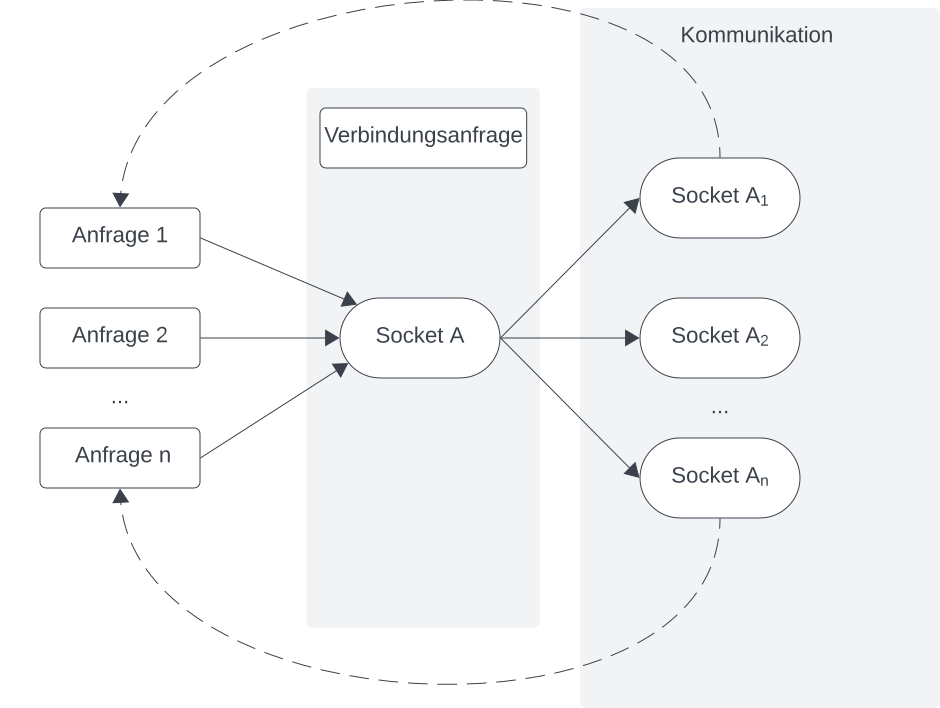
\includegraphics[scale=0.5]{chapters/fopt5/img/sockets/tcpsockets}
    \caption{Von einem TCP-Socket angenommene Verbingungsanfragen führen zu neuen Sockets, die letztendlich für die Kommunikation mit den Clients verantwortlich sind. (Quelle: eigene)}
    \label{fig:tcpsockets}
\end{figure}



\noindent
$\rightarrow$ für einen Port kann es somit mehrere Sockets geben.\\

Beispiel für eine Programmstruktur für eine Kommunikation zwischen UDP-Client und -Server:
\begin{minted}[mathescape,
    linenos,
    numbersep=5pt,
    gobble=2,
    frame=lines,
    framesep=2mm]{java}
    // TCP Client
    c = ErzeugeTCPSocket();
    baue über c eine Verbindung zu ServerAdresse/Portnummer auf;
    /* c ist blockiert, bis Timeout abgelaufen oder Anfrage angenommen */
    while (beliebig) {
        sende Nachricht über Socket c;
        warte auf Nachricht an Socket c;
        tue etwas mit der Nachricht;
    }
    schliesse die Verbindung über c;

    // TCP Server
    s = ErzeugeTCPSocketAnPort(port);
    while (beliebig) {
        warte auf Verbindungsanfrage an s und erstelle
        neuen Socket q;

        while (Verbindung besteht) {
            warte auf Nachricht von Client an Socket q
            wenn nachricht da ist {
                analysiere die Nachricht;
                führe Aktion aus;
                schicke über q Antwort an die Adresse/Portnummer
                der Nachricht;
            } ansonsten nach timeout oder verbindungsabbruch {
                schliesse Verbindung über q;
                verlasse die innere schleife und warte auf
                neue verbindung;
            }

        }
    }
\end{minted}\\

\noindent
Es gibt bei \textbf{TCP} höchstens eine Verbindung von einem Port auf einem Rechner zu einem anderen Port auf einen anderen Rechner, aber es können mehrere Verbindungen von einem Port zu unterschiedlichen Ports des Zielrechners existieren, bzw. es kann ein Rechner mehrere Verbindungen zu einem bestimmten Port auf einem unterschiedlichen Zielrechner erstellen (s. Abbildung~\ref{fig:tcpconnections}).


\begin{figure}
    \centering
    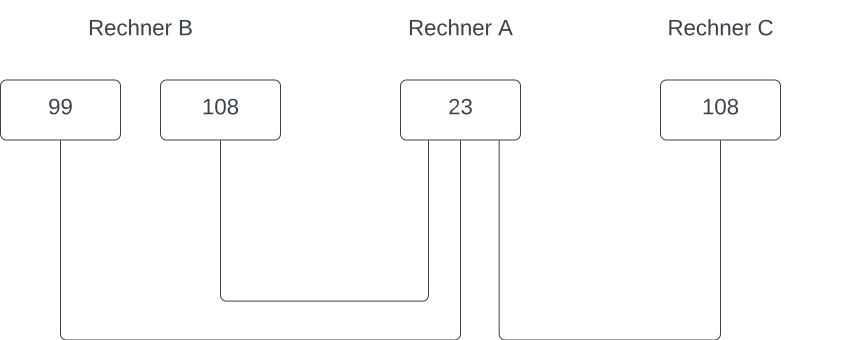
\includegraphics[scale=0.5]{chapters/fopt5/img/sockets/tcpconnections}
    \caption{Rechner $A$ bedient zweimal dieselbe Portnummer $108$ auf zwei unterschiedlichen Rechnern $B$ und $C$, von Port $23$ aus. Gleichzeitig wird Port $99$ von Rechner $B$ von Rechner $A$ bedient. (Quelle: in Anlehnung an \cite[265, Bild 5.3]{Oec22})}
    \label{fig:tcpconnections}
\end{figure}


\subsection{Socket-Schnittstelle für Java}

Die Java-Klassenbibliothek enthält u.a. im Package \code{java.net} Implementierung zur Realisierung von Socket-Kommunikation.\\

\noindent
\code{InetAddress} ist eine Klasse zur Handhabung von von Rechnernamen / IP-Adressen.\\

\noindent
\code{DatagramPacket} und \code{DatagramSocket} werden zur \textbf{UDP}-Kommunikation verwendet.\\

\noindent
\code{Socket} und \code{ServerSocket} werden zur \textbf{TCP}-Kommunikation benötigt.


